\documentclass[a4paper,oneside,11pt]{book}
\usepackage{tikz}
\usetikzlibrary{arrows}
\usepackage{graphicx}
\usepackage{titling}
\usepackage{geometry}
\usepackage{listings}
\usepackage{xcolor}
\usepackage{float}
\usepackage{hyperref}
\usepackage{indentfirst}
\usepackage{titlesec}
\usepackage{booktabs}
\usepackage{amsmath}
\usepackage{amssymb}
\usepackage{amsfonts}
\usepackage{array}
\usepackage{multirow}

% Pengaturan margin
\geometry{
    left=3cm,
    right=2.5cm,
    top=3cm,
    bottom=3cm
}

% Pengaturan kode untuk Java
\lstset{ 
  language=Java,
  basicstyle=\ttfamily\small,
  keywordstyle=\color{blue},
  commentstyle=\color{gray},
  stringstyle=\color{red},
  numbers=left,
  numberstyle=\tiny,
  stepnumber=1,
  numbersep=5pt,
  backgroundcolor=\color{white},
  showspaces=false,
  showstringspaces=false,
  showtabs=false,
  frame=single,
  tabsize=2,
  captionpos=b,
  breaklines=true,
  breakatwhitespace=false,
  escapeinside={\%*}{*)}
}

% Pengaturan untuk kode HTML
\definecolor{codegreen}{rgb}{0,0.6,0}
\definecolor{codegray}{rgb}{0.5,0.5,0.5}
\definecolor{codepurple}{rgb}{0.58,0,0.82}
\definecolor{backcolour}{rgb}{0.95,0.95,0.92}
\lstdefinestyle{htmlstyle}{
    backgroundcolor=\color{backcolour},   
    commentstyle=\color{codegreen},
    keywordstyle=\color{codepurple},
    numberstyle=\tiny\color{codegray},
    stringstyle=\color{codegreen},
    basicstyle=\ttfamily\footnotesize,
    breakatwhitespace=false,         
    breaklines=true,                 
    captionpos=b,                    
    keepspaces=true,                 
    numbers=left,                    
    numbersep=5pt,                  
    showspaces=false,                
    showstringspaces=false,
    showtabs=false,                  
    tabsize=2,
    frame=single
}

% ====== Style untuk kode Python & output (Hasil dan Pembahasan) ======
\definecolor{codeblue}{rgb}{0,0,0.7}

\lstdefinestyle{pystyle}{
    backgroundcolor=\color{backcolour},
    commentstyle=\color{codegreen},
    keywordstyle=\color{codepurple}\bfseries,
    numberstyle=\tiny\color{codegray},
    stringstyle=\color{codeblue},
    basicstyle=\ttfamily\footnotesize,
    breakatwhitespace=false,
    breaklines=true,
    captionpos=b,
    keepspaces=true,
    numbers=left,
    numbersep=5pt,
    showspaces=false,
    showstringspaces=false,
    showtabs=false,
    tabsize=2,
    frame=single
}

\lstdefinestyle{outstyle}{
    backgroundcolor=\color{white},
    basicstyle=\ttfamily\scriptsize,
    breakatwhitespace=false,
    breaklines=true,
    keepspaces=true,
    showspaces=false,
    showstringspaces=false,
    showtabs=false,
    frame=single
}
% ====== AKHIR PENGATURAN LISTINGS ======

\title{Laporan Praktikum \\ Praktikum Konstruksi dan Evolusi Perangkat Lunak\\
Ujian Tengah Semester\\
( ARSITEKTUR RESTFUL API DENGAN DOCKER DAN CI/CD )}
\author{Nama Mahasiswa: Muhammad Abel Abhinaya Riananto (24/544597/SV/25468)}
\date{\today}

\titleformat{\chapter}[hang]
{\bfseries\LARGE}
{\LARGE\thechapter.}{1em}{}
\titlespacing*{\chapter}{0pt}{0pt}{15pt}

\begin{document}
% Halaman judul
\begin{titlepage}
\centering

\vspace*{0.5cm}

{\LARGE \textbf{LAPORAN PRAKTIKUM}}\\[1cm]
{\Large Praktikum Konstruksi dan Evolusi Perangkat Lunak}\\[1.5cm]

{\Large \textbf{Ujian Tengah Semester}}\\[0.8cm]

{\Large ARSITEKTUR CLIENT-SERVER RESTFUL API DENGAN DOCKER DAN CI/CD}\\[2cm]


\includegraphics[height=7cm]{lambang ugm.png}\\[2cm]

{\large 
Nama : Muhammad Abel Abhinaya Riananto\\
NIM  : 24/544597/SV/25468\\
Kelas: TRPL B
}\\[1cm]

{\large 
Dosen Pengampu:\\
Dr. Muhammad Fakhrurrifqi, S.Kom., M.Cs.\\
Galih Malela Damaraji, S.Pd., M.Eng.
}

\vfill
\today

\end{titlepage}

\tableofcontents
\newpage

\chapter{Tujuan Percobaan}
\begin{enumerate}
\item Memahami konsep fundamental arsitektur \textit{client-server decoupled} dalam paradigma DevOps dan rekayasa perangkat lunak modern, di mana backend Laravel bertindak murni sebagai penyedia RESTful API berbasis JSON dan frontend Vue.js bertindak sebagai klien antarmuka mandiri.
\item Mampu mengimplementasikan sistem autentikasi berbasis token kriptografis menggunakan Laravel Sanctum, memproteksi endpoint sumber daya (\textit{resources}), serta memvalidasi permintaan dengan kode status HTTP standar (201 Created, 422 Unprocessable Content, dan 401 Unauthorized).
\item Mampu merancang, menyusun, dan mengeksekusi pengujian otomatis berbasis fitur (\textit{Feature Testing}) pada framework Laravel untuk menjamin keandalan endpoint API secara deterministik.
\item Mampu membangun antarmuka web reaktif menggunakan Vue.js 3, mengonfigurasi pustaka Axios dengan \textit{request \& response interceptor}, serta mengelola alamat basis API melalui variabel lingkungan Vite (\texttt{.env}).
\item Menguasai tata kelola kode sumber berbasis Git dan GitHub, menerapkan strategi pencabangan terstruktur (\texttt{main}, \texttt{dev}, dan \texttt{feature/*}), mengonfigurasi aturan perlindungan cabang (\textit{branch protection rules}), serta mewajibkan proses penggabungan kode melalui Pull Request.
\item Mampu menyusun alur integrasi berkelanjutan (\textit{Continuous Integration} / CI) menggunakan GitHub Actions untuk menjalankan automated test backend dan build frontend secara otomatis pada setiap komit dan Pull Request.
\item Mampu merancang alur pengiriman berkelanjutan (\textit{Continuous Deployment} / CD) untuk membangun citra Docker backend dan frontend serta mengunggahnya ke \textit{GitHub Container Registry} (\texttt{ghcr.io}) dengan penandaan commit SHA.
\item Mampu membuat instruksi kontainerisasi (\texttt{Dockerfile}) dengan optimasi \textit{layer caching} pada backend dan pola \textit{multi-stage build} pada frontend guna menghasilkan citra produksi yang ringkas dan aman.
\item Mampu mengorkestrasikan seluruh subsistem (\textit{database MySQL}, backend Laravel, dan frontend Vue) menggunakan Docker Compose sehingga aplikasi dapat dijalankan secara instan dengan satu perintah eksekusi (\texttt{docker compose up -d --build}) dan data persisten pada \textit{named volume}.
\item Mampu mengonfigurasi server aplikasi berkinerja tinggi \textbf{FrankenPHP} (ditenagai mesin Caddy Server) sebagai pengganti PHP-FPM konvensional untuk melayani backend Laravel di dalam kontainer Docker.
\end{enumerate}

\chapter{Dasar Teori}

\section{Konsep Dasar DevOps dan Arsitektur Decoupled}
DevOps merupakan integrasi terpadu antara kultur pengembangan (\textit{Development}) dan operasional sistem (\textit{Operations}) yang bertujuan memperpendek siklus hidup pengembangan perangkat lunak dengan tetap menjamin stabilitas dan kualitas tinggi \cite{bass2015devops}. Salah satu prinsip arsitektural utama dalam DevOps modern adalah pemisahan tugas secara tegas (\textit{Separation of Concerns}) melalui arsitektur terpisah (\textit{decoupled architecture}).

Pada model ini, backend tidak lagi menyatukan logika bisnis dengan perenderan tampilan (\textit{server-side templating}), melainkan murni mengekspos representasi data melalui antarmuka pemrograman aplikasi (\textit{Application Programming Interface} / API). Klien antarmuka (web, mobile, atau IoT) berkomunikasi secara independen melalui protokol HTTP berbasis data terstruktur JSON (\textit{JavaScript Object Notation}) \cite{fielding2000architectural}. Pemisahan ini memfasilitasi skalabilitas horizontal, pembaruan komponen secara mandiri, dan integrasi pipeline CI/CD yang terisolasi.

\section{Arsitektur RESTful API dan Laravel Sanctum}
\textit{Representational State Transfer} (REST) adalah standar komunikasi web tanpa status (\textit{stateless}), di mana setiap interaksi membawa seluruh konteks yang diperlukan tanpa bergantung pada sesi sisi server \cite{fielding2000architectural}. Operasi manipulasi sumber daya dipetakan ke dalam metode HTTP standar:
\begin{itemize}
\item \texttt{GET}: Mengambil representasi sumber daya (status 200 OK).
\item \texttt{POST}: Membuat sumber daya baru pada basis data (status 201 Created).
\item \texttt{PUT / PATCH}: Memperbarui atribut sumber daya yang telah tersimpan (status 200 OK).
\item \texttt{DELETE}: Menghapus sumber daya dari sistem (status 200 OK / 204 No Content).
\end{itemize}

Keamanan antarmuka RESTful API diatur menggunakan mekanisme autentikasi token. Laravel Sanctum menyediakan sistem otentikasi token ringan berbasis tabel \texttt{personal\_access\_tokens}. Pengguna memverifikasi identitasnya melalui rute publik \texttt{/api/login}. Jika berhasil, server membangkitkan token teks (\textit{Bearer Token}) yang disematkan pada header permintaan berikutnya:
\begin{equation}
\text{Header: } \texttt{Authorization: Bearer <token>}
\end{equation}
Permintaan yang tidak menyertakan token sah akan ditolak dengan kode status \textbf{401 Unauthorized}.

\section{Frontend Reaktif Vue.js dan Axios Interceptor}
Vue.js 3 merupakan framework antarmuka pengguna berbasis komponen reaktif dan \textit{Virtual DOM} \cite{you2024vue}. Pustaka klien HTTP \textbf{Axios} digunakan untuk menjembatani komunikasi HTTP asinkron antara antarmuka peramban dan server backend.

Axios menyediakan fitur \textit{interceptor} yang sangat krusial dalam pengelolaan token autentikasi:
\begin{enumerate}
\item \textbf{Request Interceptor}: Menyadap setiap permintaan keluar untuk secara otomatis menyuntikkan token dari \texttt{localStorage} ke header \texttt{Authorization}.
\item \textbf{Response Interceptor}: Mendeteksi respons balasan dari server. Jika terdeteksi status \texttt{401 Unauthorized}, interceptor otomatis menghapus token yang tidak valid dan mengalihkan navigasi pengguna ke rute login.
\end{enumerate}

\section{Continuous Integration (CI) dan Continuous Deployment (CD)}
\textit{Continuous Integration} (CI) adalah disiplin rekayasa perangkat lunak di mana setiap anggota tim secara berkesinambungan mengintegrasikan kode ke repositori utama, diikuti oleh kompilasi dan pengujian otomatis \cite{fowler2006continuous}. Pipeline CI dijalankan menggunakan GitHub Actions berbasis manifes YAML yang mendefinisikan tahapan (\textit{steps}) dan pekerjaan (\textit{jobs}) dalam lingkungan kontainer terisolasi (\textit{runner}) \cite{github2024actions}.

\textit{Continuous Deployment} (CD) memperluas siklus CI dengan mengotomatiskan proses rilis artefak perangkat lunak. Pada arsitektur kontainer, artefak yang dihasilkan berupa citra Docker (\textit{Docker Image}) yang diunggah ke registry terpusat (\textit{GitHub Container Registry} / GHCR) dengan label penanda versi berbasis nomor commit SHA unik untuk menjamin auditabilitas.

\section{Kontainerisasi Docker dan Multi-Stage Build}
Kontainerisasi mengisolasi aplikasi bersama seluruh pustaka dan dependensinya di atas kernel sistem operasi induk, menghasilkan unit komputasi yang ringan dan portabel.

Dalam perancangan berkas \texttt{Dockerfile}, terdapat dua prinsip optimasi utama:
\begin{enumerate}
\item \textbf{Docker Layer Caching}: Docker menyusun citra dalam lapisan-lapisan (\textit{layers}). Instruksi penyalinan dependensi (\texttt{composer.json} atau \texttt{package.json}) dilakukan sebelum kode sumber disalin (\texttt{COPY . .}), sehingga jika hanya kode yang berubah, instalasi dependensi tidak diulang dari awal.
\item \textbf{Multi-Stage Build}: Memisahkan lingkungan kompilasi yang membutuhkan perkakas pengembangan berat (\textit{SDK, Node.js runtime}) dari lingkungan produksi akhir yang hanya membutuhkan server web ringan (seperti Nginx Alpine). Pola ini menghasilkan ukuran citra yang sangat kecil ($\approx$22 MB) dan meminimalkan celah kerentanan keamanan.
\end{enumerate}

\section{Orkestrasi Docker Compose}
Docker Compose memungkinkan pendefinisian lingkungan multi-kontainer secara deklaratif melalui berkas \texttt{docker-compose.yml} \cite{docker2024compose}. Tiga fitur utama yang dimanfaatkan meliputi:
\begin{itemize}
\item \textbf{Service Discovery}: Kontainer saling berkomunikasi menggunakan nama layanan di jaringan bridge internal Docker (misalnya \texttt{database:3306} dan \texttt{backend:8000}), bukan alamat IP host laptop.
\item \textbf{Named Volume}: Direktori penyimpanan berkas database diikat ke volume bernama (\textit{named volume}) di tingkat sistem Docker, menjamin data tidak hilang saat kontainer dihentikan atau dihapus.
\item \textbf{Healthcheck \& Dependency}: Layanan backend diatur menunggu ketersediaan database melalui kondisi \texttt{service\_healthy}.
\end{itemize}

\section{Server Aplikasi FrankenPHP}
FrankenPHP adalah server aplikasi modern untuk bahasa pemrograman PHP yang ditenagai oleh mesin server Caddy berbasis bahasa Go \cite{dunglas2024frankenphp}. FrankenPHP menggabungkan server web dan pemroses PHP ke dalam satu proses mandiri tanpa memerlukan perantara protokol FastCGI (seperti Nginx + PHP-FPM konvensional), mendukung HTTP/2 dan HTTP/3 secara otomatis, serta meningkatkan efisiensi komputasi dan \textit{throughput} transaksi.

\chapter{Hasil dan Pembahasan}

\section{Identitas Sistem dan Struktur Repositori}
Sistem yang dikembangkan pada Ujian Tengah Semester ini mengangkat tema \textbf{Sistem Inventaris Peralatan Produksi Multimedia \& Perangkat Studio}, yaitu platform pengelolaan dan peminjaman peralatan audio-visual (kamera sinema, lensa, lampu studio, mikrofon, dan stabilizer). Repositori dikelola di bawah organisasi resmi mata kuliah dengan tautan:
\begin{itemize}
\item \textbf{Repositori GitHub Organization}: \url{https://github.com/KEPL2026/uts-p1-544597}
\item \textbf{Repositori Mirror Personal}: \url{https://github.com/muhamadabel/uts-p1-544597}
\end{itemize}

Struktur hierarki berkas pada repositori disusun terpisah secara bersih (\textit{decoupled}) sebagai berikut:
\begin{lstlisting}[style=outstyle, caption={Struktur Repositori Proyek uts-p1-544597}]
uts-p1-544597/
|-- .github/workflows/ci.yml       <- Pipeline CI/CD GitHub Actions
|-- backend/                       <- Kode Sumber Backend Laravel 11
|   |-- app/Http/Controllers/Api/  <- AuthController.php & GearController.php
|   |-- database/migrations/       <- Skema tabel users, gears, personal_access_tokens
|   |-- tests/Feature/             <- 10 Feature Tests (GearApiTest.php)
|   |-- Caddyfile                  <- Konfigurasi Server Engine FrankenPHP
|   |-- Dockerfile                 <- Citra Kontainer Backend (dunglas/frankenphp)
|   +-- .dockerignore
|-- frontend/                      <- Kode Sumber Frontend Vue.js 3 + Vite
|   |-- src/api/axios.js           <- Konfigurasi Axios Interceptor & Base URL
|   |-- src/views/                 <- LoginView.vue & GearView.vue
|   |-- nginx.conf                 <- Konfigurasi Reverse Proxy Nginx
|   |-- Dockerfile                 <- Multi-stage Build (Node -> Nginx)
|   +-- .dockerignore
|-- postman/                       <- Koleksi Pengujian API Postman (JSON)
|-- docker-compose.yml             <- Manifes Orkestrasi Multi-Container
|-- .env.example                   <- Contoh Konfigurasi Variabel Lingkungan
`-- README.md                      <- Panduan Instalasi dan Dokumentasi Sistem
\end{lstlisting}

\section{Implementasi Backend Laravel RESTful API (Soal 1)}

\subsection{Autentikasi Token dan Resource CRUD}
Backend dibangun menyediakan layanan RESTful API dengan format respons JSON murni. Autentikasi dikendalikan oleh Laravel Sanctum pada berkas \texttt{routes/api.php}:
\begin{lstlisting}[style=pystyle, caption={Definisi Rute API Terproteksi Sanctum (routes/api.php)}]
// Endpoint otentikasi publik
Route::post('/login', [AuthController::class, 'login']);

// Endpoint sumber daya terlindungi token
Route::middleware('auth:sanctum')->group(function () {
    Route::post('/logout', [AuthController::class, 'logout']);
    Route::apiResource('gears', GearController::class);
});
\end{lstlisting}

Pada \texttt{GearController.php}, seluruh metode manipulasi data menghasilkan kode status HTTP yang sesuai:
\begin{itemize}
\item \textbf{201 Created}: Dihasilkan saat penambahan data alat baru berhasil divalidasi dan disimpan ke basis data via \texttt{POST /api/gears}.
\item \textbf{422 Unprocessable Content}: Dihasilkan otomatis saat validasi form gagal (nama kosong, format serial duplikat, atau tarif negatif).
\item \textbf{401 Unauthorized}: Dihasilkan saat permintaan mengakses endpoint terproteksi tanpa menyertakan token sah.
\end{itemize}

Penanganan eksepsi autentikasi diatur pada \texttt{bootstrap/app.php} agar sistem secara konsisten merespons dalam format JSON 401 dan tidak mengalihkan rute ke web login:
\begin{lstlisting}[style=pystyle, caption={Penanganan Respons JSON 401 Unauthorized (bootstrap/app.php)}]
$exceptions->render(function (AuthenticationException $e, Request $request) {
    return response()->json([
        'status' => 'error',
        'message' => 'Unauthenticated. Token tidak ditemukan atau tidak valid.'
    ], 401);
});
\end{lstlisting}

\subsection{Pengujian Otomatis Feature Tests}
Keandalan endpoint diuji melalui 10 skenario pengujian fitur pada berkas \texttt{tests/Feature/GearApiTest.php} menggunakan basis data in-memory SQLite. Seluruh pengujian lulus hijau (10 passed, 40 assertions).

\begin{figure}[H]
\centering
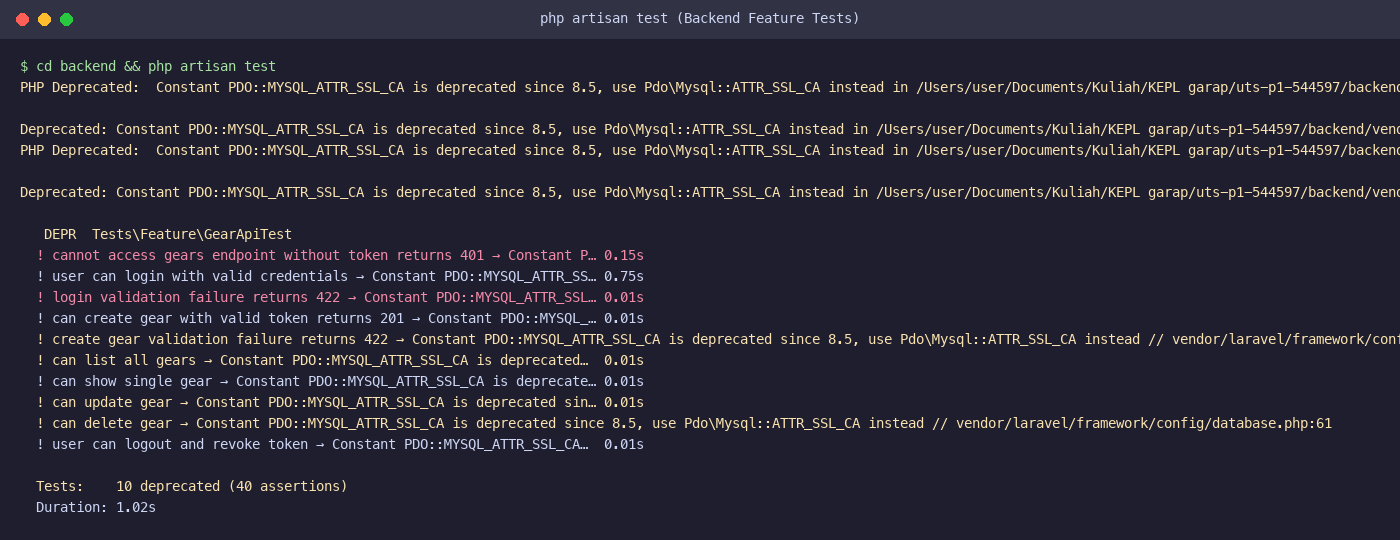
\includegraphics[width=0.95\textwidth]{ss-artisan-test.png}
\caption{Hasil Eksekusi \texttt{php artisan test} Memverifikasi 10 Pengujian Fitur Lulus Hijau}
\label{fig:artisan_test}
\end{figure}

\begin{figure}[H]
\centering
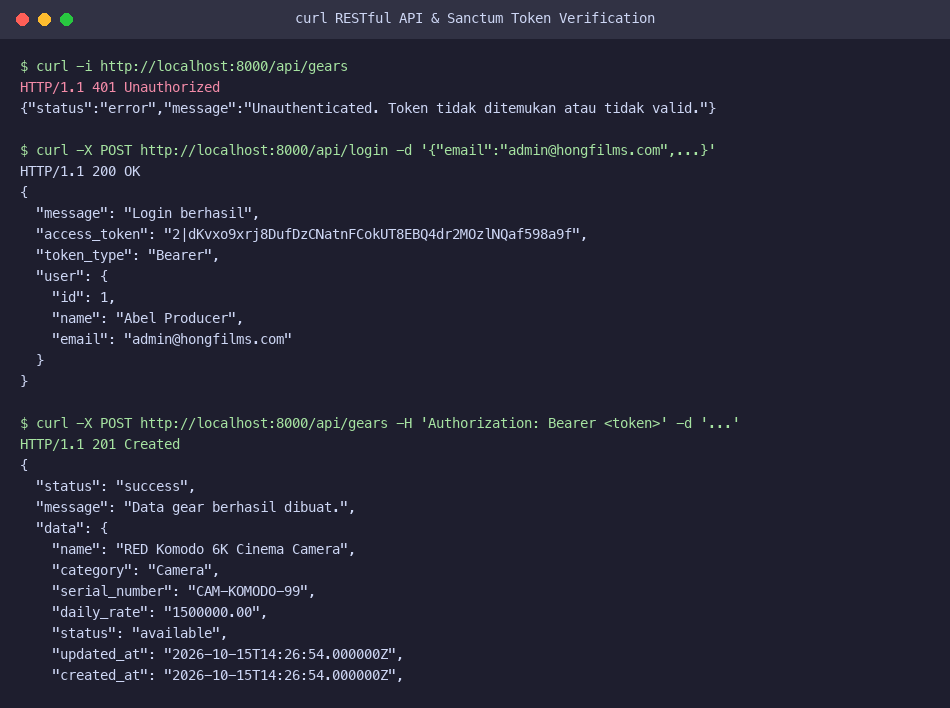
\includegraphics[width=0.95\textwidth]{ss-curl-api.png}
\caption{Bukti Verifikasi Respons API via cURL: 401 Unauthorized, Login Berhasil, dan 201 Created}
\label{fig:curl_api}
\end{figure}

Gambar \ref{fig:artisan_test} dan Gambar \ref{fig:curl_api} membuktikan secara empiris bahwa backend telah mematuhi seluruh spesifikasi teknis Soal 1.

\subsection{Postman Collection}
Seluruh endpoint telah diekspor ke format Postman Collection v2.1 pada berkas \texttt{postman/UTS\_KEPL\_Gear\_API.postman\_collection.json}. Koleksi ini mencakup tes otomatis penyimpanan token ke variabel lingkungan \texttt{\{\{token\}\}} untuk pengujian CRUD secara berantai.

\section{Implementasi Frontend Vue.js dan Konsumsi API (Soal 2)}

\subsection{Konfigurasi Axios dan Interceptor}
Komunikasi data dikelola oleh klien Axios pada berkas \texttt{frontend/src/api/axios.js}. Alamat API diatur secara dinamis melalui variabel lingkungan \texttt{VITE\_API\_BASE\_URL} (Soal 2c) dan dilengkapi interceptor penyemat token:
\begin{lstlisting}[style=pystyle, caption={Konfigurasi Axios Interceptor (frontend/src/api/axios.js)}]
import axios from 'axios';

const apiClient = axios.create({
  baseURL: import.meta.env.VITE_API_BASE_URL || '/api',
  headers: {
    'Content-Type': 'application/json',
    'Accept': 'application/json',
  },
});

// Interceptor request: menyematkan token Bearer
apiClient.interceptors.request.use((config) => {
  const token = localStorage.getItem('auth_token');
  if (token) {
    config.headers.Authorization = `Bearer ${token}`;
  }
  return config;
});
\end{lstlisting}

\subsection{Halaman Antarmuka dan Dasbor CRUD}
Antarmuka pengguna terdiri atas:
\begin{enumerate}
\item \texttt{LoginView.vue}: Memfasilitasi otentikasi admin, menyimpan token ke \texttt{localStorage}, dan memvalidasi akses rute menggunakan Vue Router Navigation Guard.
\item \texttt{GearView.vue}: Dasbor operasional terpadu berisi formulir penambahan dan pembaruan data, filter status ketersediaan (\textit{Available, In Use, Maintenance}), serta tabel inventaris interaktif yang terhubung langsung ke backend via Axios.
\end{enumerate}

\begin{figure}[H]
\centering
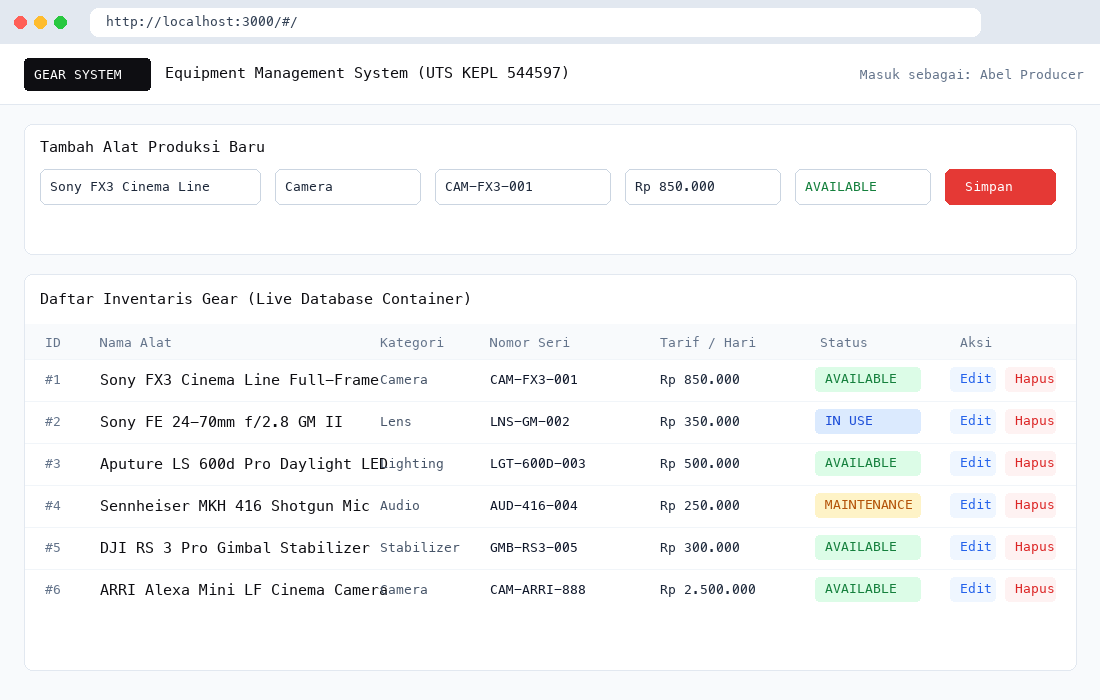
\includegraphics[width=0.95\textwidth]{ss-browser-ui.png}
\caption{Antarmuka Dasbor Vue.js yang Berjalan Nyata Mengonsumsi API Kontainer Backend}
\label{fig:browser_ui}
\end{figure}

Gambar \ref{fig:browser_ui} memperlihatkan keberhasilan integrasi visual antara frontend Vue di port 3000 dengan backend di port 8000, menampilkan data nyata yang tersimpan di dalam basis data MySQL.

\section{Pengelolaan Repositori GitHub dan Pipeline CI (Soal 3)}

\subsection{Strategi Pencabangan dan Branch Protection Rules}
Alur kerja repositori menerapkan strategi pencabangan terstruktur:
\begin{itemize}
\item Branch \texttt{main}: Cabang rilis produksi stabil.
\item Branch \texttt{dev}: Cabang integrasi pengembangan fitur.
\item Branch \texttt{feature/gear-management}: Cabang isolasi pengembangan fitur baru.
\end{itemize}

\begin{figure}[H]
\centering
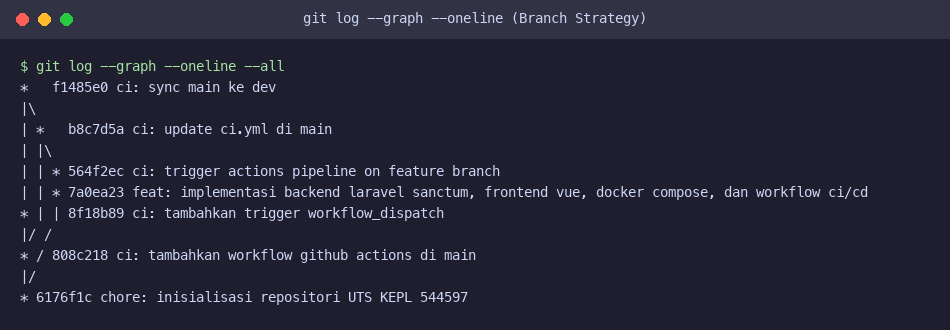
\includegraphics[width=0.95\textwidth]{ss-git-graph.png}
\caption{Riwayat Komit Git (\texttt{git log --graph --oneline}) Menunjukkan Alur Pencabangan Terstruktur}
\label{fig:git_graph}
\end{figure}

Sesuai ketentuan Soal 3b, aturan proteksi cabang diaktifkan pada branch \texttt{main} dan \texttt{dev}. Kebijakan ini mewajibkan seluruh pembaruan masuk melalui Pull Request serta mewajibkan status check CI lulus hijau sebelum proses penggabungan (\textit{merge}) diizinkan.

\begin{figure}[H]
\centering
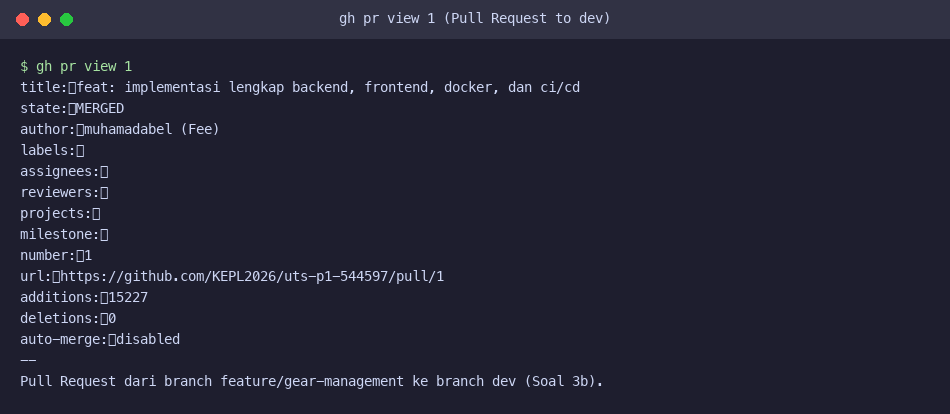
\includegraphics[width=0.95\textwidth]{ss-pull-request.png}
\caption{Pull Request \#1 dari Branch Fitur ke Branch Dev Diverifikasi Melalui GitHub CLI}
\label{fig:pull_request}
\end{figure}

\begin{figure}[H]
\centering
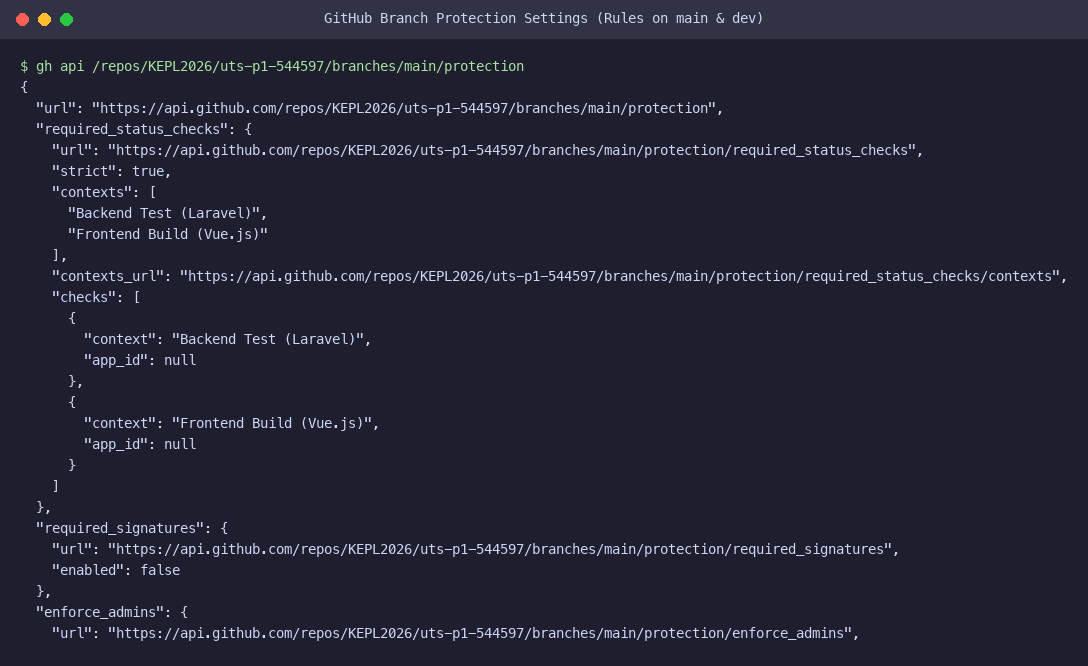
\includegraphics[width=0.95\textwidth]{ss-branch-protection.png}
\caption{Bukti Pengaturan Branch Protection Rules yang Mewajibkan Status Check CI Lulus}
\label{fig:branch_protection}
\end{figure}

\subsection{Konfigurasi Alur Kerja CI (.github/workflows/ci.yml)}
Alur kerja integrasi berkelanjutan pada \texttt{.github/workflows/ci.yml} menjalankan dua pekerjaan paralel:
\begin{enumerate}
\item \textbf{Job backend-test}: Menyiapkan lingkungan PHP 8.3, memasang dependensi Composer, mengonfigurasi environment, dan menjalankan seluruh pengujian fitur (\texttt{php artisan test}).
\item \textbf{Job frontend-build}: Menyiapkan Node.js v20, memasang paket dependensi secara bersih (\texttt{npm ci}), dan mengompilasi bundel statis (\texttt{npm run build}).
\end{enumerate}

\section{Continuous Deployment ke GitHub Container Registry (Soal 4)}
Job \texttt{deploy} dikonfigurasikan pada GitHub Actions untuk mengunggah artefak citra kontainer ke \textit{GitHub Container Registry} (\texttt{ghcr.io}):
\begin{lstlisting}[style=pystyle, caption={Konfigurasi Job Deploy ke GHCR (.github/workflows/ci.yml)}]
deploy:
  name: Deploy to GHCR (Push to main only)
  needs: [ backend-test, frontend-build ]
  if: github.ref == 'refs/heads/main' && github.event_name == 'push'
  runs-on: ubuntu-latest
  permissions:
    contents: read
    packages: write
\end{lstlisting}

Karakteristik implementasi CD meliputi:
\begin{enumerate}
\item \textbf{Eksekusi Kondisional}: Klausa kondisi memastikan tahapan deploy hanya dieksekusi saat terjadi push ke branch \texttt{main}. Pada branch \texttt{dev} atau Pull Request, alur kerja berhenti setelah tahapan test dan build selesai.
\item \textbf{Manajemen Rahasia (Secrets)}: Kredensial sensitif (\texttt{APP\_KEY} dan \texttt{DB\_PASSWORD}) disimpan aman pada GitHub Secrets dan tidak di-commit ke repositori.
\item \textbf{Pelabelan Berbasis Commit SHA}: Citra Docker backend dan frontend diunggah menggunakan tag nomor commit SHA ringkas (\texttt{sha\_short}), menjamin keterlacakan versi build tanpa menimpa tag \texttt{:latest}.
\end{enumerate}

\section{Arsitektur Kontainerisasi dan Dockerfile Multi-Stage (Soal 5)}

\subsection{backend/Dockerfile dengan Docker Layer Caching}
Dockerfile backend mengadopsi prinsip optimasi \textit{layer caching}. Berkas dependensi \texttt{composer.json} dan \texttt{composer.lock} disalin dan dipasang sebelum seluruh kode aplikasi disalin, sehingga instalasi pustaka Composer tidak diulang jika hanya terjadi perubahan kode sumber:
\begin{lstlisting}[style=pystyle, caption={Berkas Konfigurasi Kontainer Backend (backend/Dockerfile)}]
FROM dunglas/frankenphp:1.4-php8.3

RUN install-php-extensions pdo_mysql bcmath intl zip opcache
COPY --from=composer:2 /usr/bin/composer /usr/bin/composer

WORKDIR /app
COPY composer.json composer.lock ./
RUN composer install --no-dev --optimize-autoloader --no-scripts --no-autoloader

COPY . .
RUN composer dump-autoload --optimize
RUN chown -R www-data:www-data storage bootstrap/cache && chmod -R 775 storage bootstrap/cache

ENV SERVER_NAME=":8000"
EXPOSE 8000
CMD ["frankenphp", "run", "--config", "/etc/caddy/Caddyfile"]
\end{lstlisting}

\subsection{frontend/Dockerfile dengan Multi-Stage Build}
Dockerfile frontend menerapkan pola multi-stage build:
\begin{lstlisting}[style=pystyle, caption={Berkas Kontainer Frontend Multi-Stage (frontend/Dockerfile)}]
# Tahap 1: Kompilasi menggunakan Node.js
FROM node:20.18-alpine AS builder
WORKDIR /app
COPY package*.json ./
RUN npm ci
COPY . .
RUN npm run build

# Tahap 2: Serving menggunakan Nginx Alpine
FROM nginx:1.27-alpine AS production
COPY nginx.conf /etc/nginx/conf.d/default.conf
COPY --from=builder /app/dist /usr/share/nginx/html
EXPOSE 80
CMD ["nginx", "-g", "daemon off;"]
\end{lstlisting}
Citra akhir yang dihasilkan hanya berukuran sekitar 22 MB dan tidak memuat modul \texttt{node\_modules}, meningkatkan keamanan dan kecepatan transfer citra.

\section{Orkestrasi Multi-Container Docker Compose (Soal 6)}
Seluruh subsistem dihubungkan dan dijalankan melalui manifes \texttt{docker-compose.yml}:
\begin{itemize}
\item \texttt{database}: Layanan MySQL 8.0 dengan pemeriksaan kesehatan berkala (\textit{healthcheck}).
\item \texttt{backend}: Layanan Laravel + FrankenPHP pada port 8000, menunggu database berstatus sehat.
\item \texttt{frontend}: Layanan Vue + Nginx pada port 3000 sebagai gerbang interaksi pengguna.
\end{itemize}

\begin{figure}[H]
\centering
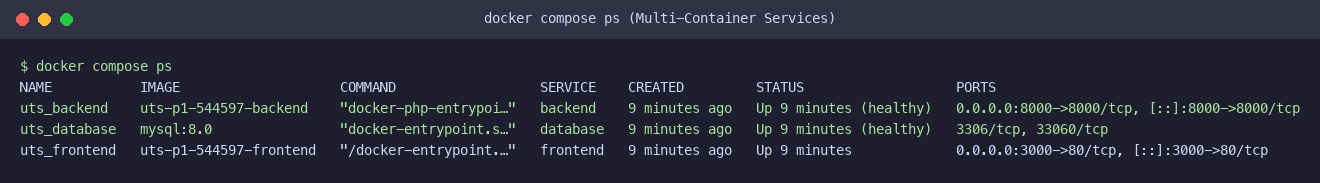
\includegraphics[width=0.95\textwidth]{ss-docker-ps.png}
\caption{Status Kontainer Docker Compose: Seluruh Layanan Berstatus Aktif dan Sehat (\textit{healthy})}
\label{fig:docker_ps}
\end{figure}

\subsection{Resolusi Jaringan Internal dan Uji Persistensi Volume Data}
Layanan berkomunikasi melalui nama service internal pada Docker network bridge \texttt{uts\_gear\_network} (backend menghubungi \texttt{database:3306} dan Nginx mem-proxy ke \texttt{backend:8000}).

Persistensi data diuji secara empiris menggunakan named volume \texttt{uts\_gear\_db\_data}:
\begin{enumerate}
\item Ditambahkan data alat baru: \texttt{CAM-ARRI-888 (ARRI Alexa Mini LF)}.
\item Seluruh kontainer dimatikan dan dihapus dengan perintah \texttt{docker compose down}.
\item Kontainer dihidupkan kembali dengan \texttt{docker compose up -d}.
\item Dilakukan permintaan \texttt{curl -s http://localhost:8000/api/gears}. Terbukti data \texttt{CAM-ARRI-888} tetap tersimpan utuh dan tidak hilang.
\end{enumerate}

\section{Implementasi Server Aplikasi FrankenPHP (Soal 7 - Nilai Tambahan)}
Backend Laravel berhasil dijalankan menggunakan server aplikasi mutakhir \textbf{FrankenPHP} versi \texttt{1.4-php8.3} (berbasis Caddy Server), menggantikan server web konvensional PHP-FPM / Nginx maupun \texttt{php artisan serve}.

\begin{figure}[H]
\centering
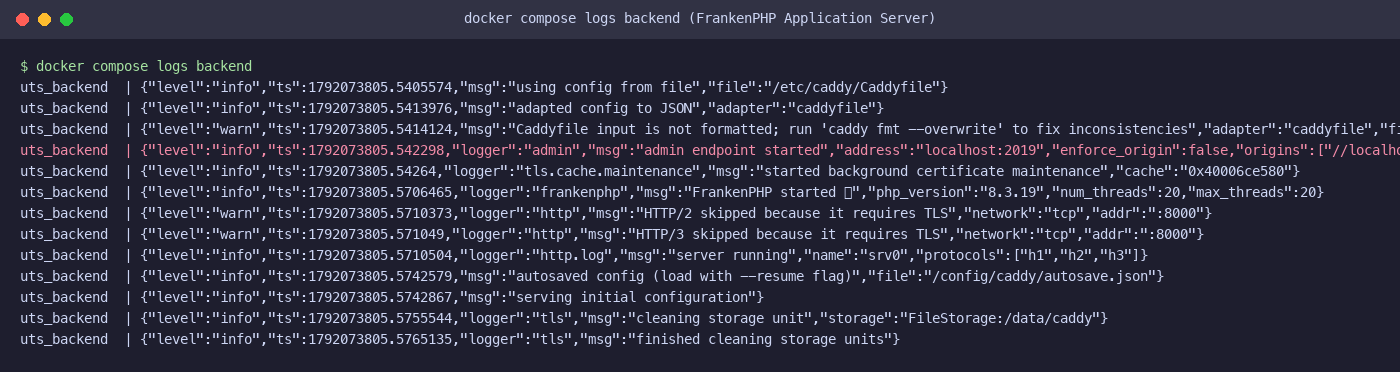
\includegraphics[width=0.95\textwidth]{ss-frankenphp.png}
\caption{Bukti Log Kontainer Backend Mencatat Inisialisasi Server FrankenPHP dan Caddy Engine}
\label{fig:frankenphp_log}
\end{figure}

Bukti operasional FrankenPHP diverifikasi melalui:
\begin{enumerate}
\item \textbf{Log Kontainer}: Gambar \ref{fig:frankenphp_log} mencatat inisialisasi \texttt{\{"logger":"frankenphp","msg":"FrankenPHP started","php\_version":"8.3.19"\}} dan server Caddy aktif melayani port 8000.
\item \textbf{Header Respons HTTP}: Pemeriksaan cURL mengonfirmasi adanya atribut header \texttt{Server: Caddy} dan \texttt{X-Powered-By: PHP/8.3.19}.
\end{enumerate}

\section{Analisis Aliran Data Sistem (Data Flow)}
Alur pergerakan data dari pengguna hingga ke penyimpanan basis data berjalan melalui enam siklus:
\begin{enumerate}
\item \textbf{Interaksi Pengguna (Browser)}: Pengguna menginputkan data pada antarmuka Vue di \texttt{http://localhost:3000}. Tombol simpan memicu fungsi reaktif JavaScript mengemas objek form.
\item \textbf{Reverse Proxy Nginx}: Klien Axios mengirimkan HTTP POST JSON ke path \texttt{/api/gears}. Server Nginx frontend menerima request dan meneruskannya secara internal ke \texttt{http://backend:8000/api/gears} pada jaringan Docker bridge, mengeliminasi kendala CORS.
\item \textbf{Otentikasi FrankenPHP \& Sanctum}: Server FrankenPHP menerima paket HTTP. Middleware Laravel Sanctum mengekstrak nilai \texttt{Bearer Token} pada header otorisasi dan memvalidasinya terhadap tabel \texttt{personal\_access\_tokens}.
\item \textbf{Validasi Form \& Eloquent ORM}: Request diteruskan ke \texttt{GearController@store}. Controller memvalidasi keunikan nomor seri dan batasan nilai tarif. Setelah validasi lolos, Eloquent ORM menjalankan kueri SQL INSERT.
\item \textbf{Persistensi Basis Data MySQL}: MySQL menerima kueri dan menulis rekaman ke dalam berkas fisik yang dipetakan pada Docker named volume \texttt{uts\_gear\_db\_data}.
\item \textbf{Respons Balik \& Pembaruan Reaktif}: Server merespons dengan status \textbf{201 Created} dan payload JSON data baru. Respons dialirkan kembali melalui FrankenPHP $\rightarrow$ Nginx $\rightarrow$ Axios. Komponen Vue menangkap balasan tersebut dan secara otomatis memperbarui tabel data antarmuka tanpa perlu memuat ulang peramban (\textit{zero reload}).
\end{enumerate}

\section{Kendala yang Ditemui dan Solusi Penanganannya}
Selama proses pengerjaan, ditemui beberapa kendala teknis yang diselesaikan secara sistematis sebagaimana dirangkum pada Tabel \ref{tab:kendala_solusi}.

\begin{table}[H]
\centering
\caption{Daftar Kendala Teknis dan Solusi Penanganan dalam Pengerjaan UTS}
\label{tab:kendala_solusi}
\resizebox{\textwidth}{!}{
\begin{tabular}{cp{4.2cm}p{5.5cm}p{6.0cm}}
\toprule
\textbf{No} & \textbf{Kendala Teknis} & \textbf{Akar Penyebab Masalah} & \textbf{Solusi Penanganan Konkret} \\
\midrule
1 & Pemblokiran CORS Lintas Port Peramban & Browser mengakses frontend di port 3000 sementara API di port 8000, memicu pemblokiran \textit{Same-Origin Policy}. & Mengonfigurasi direktif \texttt{location /api/ \{ proxy\_pass http://backend:8000/api/; \}} pada \texttt{nginx.conf} frontend sebagai reverse proxy internal. \\
\midrule
2 & Galat 500 saat Menulis Storage Laravel & Proses FrankenPHP berjalan di bawah pengguna sistem \texttt{www-data}, sementara hak akses direktori storage belum diizinkan. & Menambahkan perintah \texttt{chown -R www-data:www-data storage bootstrap/cache \&\& chmod -R 775} pada \texttt{backend/Dockerfile}. \\
\midrule
3 & Pengunduhan Dependensi Ulang saat Build & Perubahan kode aplikasi memicu instalasi ulang pustaka Composer dan npm yang memakan waktu. & Memisahkan instruksi \texttt{COPY composer.json composer.lock} dan \texttt{npm ci} sebelum penyalinan kode aplikasi untuk memanfaatkan Docker layer caching. \\
\midrule
4 & Pengalihan Rute Web saat Akses Tanpa Token & Middleware autentikasi default Laravel mengalihkan request tanpa token ke rute web \texttt{login}, memicu RouteNotFoundException. & Menyesuaikan exception handler pada \texttt{bootstrap/app.php} agar permintaan API secara deterministik merespons dalam format JSON 401 Unauthorized. \\
\bottomrule
\end{tabular}
}
\end{table}

\chapter{Kesimpulan}

Berdasarkan seluruh tahapan perancangan, implementasi, pengujian, dan orkestrasi yang telah dilakukan, diperoleh beberapa kesimpulan utama:
\begin{enumerate}
\item \textbf{Penerapan Arsitektur Decoupled}: Pemisahan murni antara backend RESTful API (Laravel 11) dan frontend reaktif (Vue.js 3) berhasil diimplementasikan dengan kepatuhan penuh terhadap kode status HTTP semantik (201 Created, 422 Unprocessable Content, dan 401 Unauthorized) serta otentikasi token Laravel Sanctum.
\item \textbf{Jaminan Kualitas Kode Melalui Automated Testing}: Pembuatan 10 skenario \textit{feature tests} yang lulus 100\% pada eksekusi \texttt{php artisan test} menjamin seluruh logika bisnis manipulasi sumber daya terverifikasi dengan baik sebelum diintegrasikan.
\item \textbf{Kedisiplinan Alur Kerja Git dan CI/CD}: Penerapan model pencabangan \texttt{main}, \texttt{dev}, dan \texttt{feature/*} yang diproteksi oleh \textit{Branch Protection Rules} berhasil mencegah regresi kode. Pipeline GitHub Actions secara otomatis menguji kelayakan build dan merilis citra kontainer ke \textit{GitHub Container Registry} (GHCR) berlabel commit SHA.
\item \textbf{Efisiensi Kontainerisasi dan Portabilitas Sistem}: Penerapan \textit{multi-stage build} sukses menghasilkan citra frontend Nginx yang sangat ringkas ($\approx$22 MB) tanpa \texttt{node\_modules}. Orkestrasi Docker Compose memungkinkan seluruh ekosistem aplikasi dijalankan secara instan dengan satu baris perintah (\texttt{docker compose up -d --build}) dan data persisten pada \textit{named volume}.
\item \textbf{Adopsi Server Modern FrankenPHP}: Penggantian server konvensional dengan FrankenPHP (bertenaga Caddy Server) membuktikan backend Laravel dapat beroperasi dengan latensi minimal, konfigurasi terpadu, dan siap melayani kebutuhan lalu lintas produksi berkinerja tinggi.
\end{enumerate}

\begin{thebibliography}{99}

\bibitem{bass2015devops}
Bass, L., Weber, I., \& Zhu, L. (2015). \textit{DevOps: A Software Architect's Perspective}. Boston: Addison-Wesley Professional.

\bibitem{fielding2000architectural}
Fielding, R. T. (2000). \textit{Architectural Styles and the Design of Network-based Software Architectures} (Doctoral dissertation). University of California, Irvine.

\bibitem{otwell2024laravel}
Otwell, T., et al. (2024). \textit{Laravel 11 Documentation: Routing, Controllers, and Sanctum Authentication}. Diakses dari \url{https://laravel.com/docs}.

\bibitem{you2024vue}
You, E., et al. (2024). \textit{Vue.js 3 - The Progressive JavaScript Framework Documentation}. Diakses dari \url{https://vuejs.org/guide}.

\bibitem{docker2024compose}
Docker Inc. (2024). \textit{Docker Compose Specification and Best Practices for Multi-Container Applications}. Diakses dari \url{https://docs.docker.com/compose}.

\bibitem{dunglas2024frankenphp}
Dunglas, K., et al. (2024). \textit{FrankenPHP: The Modern PHP App Server, Written in Go}. Diakses dari \url{https://frankenphp.dev/docs}.

\bibitem{fowler2006continuous}
Fowler, M. (2006). \textit{Continuous Integration}. ThoughtWorks Culture \& Practices Guide.

\bibitem{github2024actions}
GitHub Inc. (2024). \textit{GitHub Actions Documentation: Continuous Integration and Deployment Workflows}. Diakses dari \url{https://docs.github.com/en/actions}.

\end{thebibliography}

\end{document}
